%!TEX program = lualatex
\documentclass[14pt]{constructor-diploma}

\usepackage[backend=bibtex]{biblatex}
\addbibresource{diploma.bib}

\begin{document}
\filltitle{en}{
    chair              = {Bachelor of Science \\ Computer Science},
    title              = {Equality saturation for solving equalities of relational expressions},
    author             = {Andrei Kozyrev},
    supervisorPosition = {professor},
    supervisor         = {Anton Podkopaev},
    reviewerPosition   = {},
    reviewer           = {},
    chairHeadPosition  = {professor},
    chairHead          = {Christobal Junta},
}
\maketitle

\emptypage{}
\section*{Abstract}
Modern CPUs are being developed exceptionally fast, and the number of cores is increasing rapidly. This has led to the development of multithreading, which is a technique that allows for the execution of multiple threads on a single CPU.\@ Memory models are a fundamental aspect of multithreading and describe how memory is ordered at runtime in relation to source code. Currently, existing memory models are unsatisfactory and there is a need for new models that can be rigorously proven. In order to achieve this, formal verification using the Coq proof assistant is utilized, which enables automated proof checking and ensures the accuracy of results. Specialists in weak memory are continuosly improving the results in this domain.

One of the big and common problems in weak memory is the proof of equivalence of several memory models. Memory models are represented as expressions over relational language. 

This thesis focuses on the automation of proving equalities over relational expressions in Coq.\@ We are utilizing the techniques of equality saturation and E-graph data structure to generate proof of equaivalence for a given pair of terms. By automating these proofs, we can greatly increase the efficiency and accuracy of the proof process in weak memory.
\emptypage{}
\section*{Acknowledgements}
% I would like to express my sincere gratitude to my dear friend Ivan Kabashniy for his unwavering support throughout the completion of my bachelor thesis on Equality saturation for solving equalities of relational expressions. Ivan's emotional support played a crucial role in keeping me motivated and focused during the challenging moments of my research journey. His kind words, encouragement, and patience helped me overcome the hurdles that I encountered and kept me on track towards achieving my academic goals. I am deeply grateful to Ivan for being a constant source of inspiration and for always believing in me. Thank you, Ivan, for your invaluable friendship and for being a significant part of my academic success.

\lipsum[1]

\emptypage{}
\tableofcontents

\include{chapters/1-introduction}
\newpage
\section{Objectives}
This thesis aims to automate solving equaivalences over relational expressions in Coq. The goal is to manage to use the \texttt{egg} library and automate the proof process. The main objectives are:
\begin{itemize}
    \item Develop a framework for communication between Rust and the \texttt{Coq} interactive proofs. We need to connect two completely stadalone systems, Coq and \texttt{egg}, together to enable their communication and data interchange.
    % TODO: Add reference to the chapter. 
    \item Make a rule-parameterized algorithm on top of the \texttt{egg} library for producing a series of rewrites, which prove relational equivalence. Given two expressions and a rewriting system, there may be multipl eapproaches to prove the equivalence. The naive approach to build an e-graph for one expression and search for another may have problems unrevealed in Chapter {?}. 
    \item Experiment on existing proofs and used lemmas to come up with a usable and efficient rule set. Firstly, to analyse existing weak memory proofs and provide users a useful interface. Secondly, as big rule sets result in huge e-graphs, that take long to be built, we aim to research on the efficient and substantive rule set, that would be small enough to be used to build e-graphs in practice.
\end{itemize}
\newpage
\section{Related Work}
First part of this chapter focuses on introducing the reader to Coq proof assistant, its core concepts and significance. Then other solutions to the problem are discussed in Section~\ref{othersoulutions}. Finally, we focus on the details of our particular approach and cover details regarding equality saturation and the \texttt{egg} library in Section~\ref{egraphs}.

\subsection{Coq}\label{relatedworkcoq}
This section aims to provide an overview of Coq and its significance in the field of theorem proving. We will outline the advantages of using Coq compared to other proof assistants and methods. Additionally, we will delve deeper into the Coq proving process.

\subsubsection{Coq Overview}
% TODO: Попробовал добавить footnote на терминал, выглядит как степень...
Coq is a formal proof management system. It provides a language called Gallina, which is used to define mathematical objects and write formal proofs. The formalism behind Coq is the Calculus of Inductive Constructions (CIC)~\cite{paulinmohring:hal-01094195}. In CIC types are used to ensure the correctness of proofs. Each theorem is essentially a type, and its proof is a value inhabiting that type. It might also be useful to think of proofs as functions from hypothesis to conclusion. For example, assume we have a context $\Gamma$, a proposition $\varphi$ and we want to prove $\Gamma \vdash \varphi$. That would mean that the proof we are looking for is a mapping, which for any argument of type $\Gamma$ constructs a value of type $\varphi$. 

\subsubsection{Coq Proof mode}
As mentioned earlier, proofs can be viewed as functions and this is one of the ways to make a proof in Coq. We will provide an example for a better understanding. Consider the following theorem: given value of type $A$ and a function $f : A \to B$, we can construct a value of type $B$. 

\vspace{0.5cm}
\begin{lstlisting}[language=coq]
    Definition test (A B : Prop) :
      A -> (A -> B) -> B.
\end{lstlisting}

To prove such theorem we need to apply the value $a$ of type $A$ to the function $f$ and conclude the proof:

\vspace{0.5cm}
\begin{lstlisting}[language=coq]
    Definition test (A B : Prop) :
      A -> (A -> B) -> B
    := fun (a : A) (f : A -> B) => f a.
\end{lstlisting}

Constracting proof terms by hand may be useful to learn Coq, but it is very inconvenient to write bigger proofs in such manner. In a bigger proof, as like as in paper proofs, you want to iteratively modify the environment and step by step achieve the goal. Coq enters proof mode when you begin a proof, such as with the \texttt{Theorem} command: 

\vspace{0.5cm}
\begin{lstlisting}[language=coq]
    Theorem test (A B : Prop) :
      A -> (A -> B) -> B.
    Proof.
\end{lstlisting}

When you enter a proof mode, you are able to always see current unfinished goals and an up-to-date hypothesises: 

\vspace{0.5cm}
\begin{lstlisting}[language=coq]
    A, B : Prop
    ============================
    A -> (A -> B) -> B
\end{lstlisting}

Now we can proof the theorem using tactics. Tactics implement backwards reasoning, so when tactic is applied, all hypothesises it uses to modify the goal are added to the context. 

Firstly, we call an \texttt{intros} tactic, which introduces all propositions on the left side of the implication as assumptions: 

\vspace{0.5cm}
\begin{lstlisting}[language=coq]
    A, B : Prop
    H : A
    H0 : A -> B
    ============================
    B
\end{lstlisting}

We have a hypothesis $H$ of type $A$, but we need $B$. We call an \texttt{apply H0} tactic, which proves us $B$, but adds $A$ as a new goal. Now if we call \texttt{apply H}, we will conclude the proof. 

\vspace{0.5cm}
\begin{lstlisting}[language=coq]
Lemma test' (A B : Prop) :
  A -> (A -> B) -> B.
Proof.
  intros.
  apply H0.
  apply H.
Qed.
\end{lstlisting}

\subsubsection{Coq's Significance}
There are other Proof Assistants continuing to appear, but Coq has been developed and improved since 1989. The heart of a proof assistant is its kernel, which is the primary source of reliability of the tool. Unfortunately, regarding of the kernel's size, as any other software, it has issues. However, the amount of work done by the Coq community to recheck and validate the kernel, makes Coq the most trustworthy proof assistant available.

% TODO: Возможно лучше заменить на Odd Order Theorem
Moreover, Coq's huge strength is the amount of impressive results, obtained using it. The most famous result, achieved using Coq, is the Four Color Theorem proof. The Four Color Theorem states that any map can be colored using only four colors, so that no two adjacent regions are colored the same. There were several paper proofs, that were all proven to be incorrect after a while. A computer-assisted proof was proposed by Kenneth Appel and Wolfgang Haken in 1976~\cite{appel_4color1976}. The proof reduced the problem to the analysis of a smaller number of options and their enumeration by a computer for many hours. Consequently, the mathematical community was not inclined to trust the proof. The first formal checked proof was proposed by George Gonthier et al.\ in 2005~\cite{Gonthier2008FormalPF}, which showed the community that Coq is ready for huge and complex proofs. 

\subsubsection{Proof Automation}
This thesis focuses on automating the proofs, whilst a question may arise whether such approach makes proofs less clear to read. There are several proof styles in Coq. A framework called \texttt{SSReflect}\footnote{\href{https://coq.inria.fr/refman/proof-engine/ssreflect-proof-language.html}{https://coq.inria.fr/refman/proof-engine/ssreflect-proof-language.html}} exists. Conceptually, \texttt{SSReflect} differs from ordinary \texttt{Tactics}\footnote{\href{https://coq.inria.fr/refman/proof-engine/tactics.html\#tactics}{https://coq.inria.fr/refman/proof-engine/tactics.html\#tactics}} in that proofs are written with almost no automation, and the tactics language is much more expressive. Even though \texttt{SSReflect} has less automation, proofs anyway tend to be confusing. From the other hand, when classical Coq \texttt{Tactics} are used, proof is usually broken down into a huge number of lemmas and sub-claims, definitions of which make the idea clear. Lemmas that are deep down inside the proof can typically be automated without sacrificing the readability, because their proofs are self-evident. 

\subsection{Alternative solutions to solving relational equations}\label{othersoulutions}
In 2023 Kokologiannakis et al.\ presented the tool called \texttt{Kater}~\cite{kater}. \texttt{Kater} is a tool that allows to automatically answer memory-model questions. \texttt{Kater} is a useful, but standalone tool. Firstly, that means we must believe in its correctness, whereas any functionality integrated into Coq is protected by the Coq's typechecker from producing incorrect results. Secondly, proofs in weak memory are ofter more diverse than just reasoning about relational expressions. For instance, we may want to prove correctness of the compilation scheme, e.g.\ from C to Assembly language. In such cases, the semantics of the assembly code must be related to the original operational semantics of the instructions in our language. While relations are still relevant, they are only a small part of the problem. The main focus is on proving properties about the compilation process. Therefore, \texttt{Kater} is suitable only for a limited set of problems, where relations are the primary concern, and the proof process does not involve other complex components. In contrast, Coq provides a comprehensive framework for formal reasoning that allows us to tackle a wide range of problems. 

\subsection{E-graphs and Equality Saturation}\label{egraphs}
E-graphs are a generalization of a set-union data structure~\cite{tarjan_1975}. \\ E-graphs were first introduced by Greg Nelson and Derek C. Oppen in 1980~\cite{nelson_1980}. Since then, e-graphs have been used for a successful mechanical theorem proving and program verification, e.g.\ in Stanford Pascal Verifier at 1979~\cite{pascal_verifier_manual_1979}. 

We will now formally define an e-graph. Let $\Sigma$ be a set of function symbols. Let $\Sigma_n$ be a subset of $\Sigma$ consisting of symbols of arity $n$. Let $\operatorname{Id}$ be a set of unique idetnifiers $\operatorname{id}_1, \operatorname{id}_2, \dots, \operatorname{id}_k$, called the e-class \textbf{Id}s. Then \textbf{e-node} is a function symbol $f \in \Sigma$ and a list of $n$ e-class Ids. E-node is denoted $f(\operatorname{id}_1, \operatorname{id}_2, \dots, \operatorname{id}_n)$. E-class is a set of e-nodes. E-graph is a Disjoint Set Union data structure over e-class Ids. Here we give an example of a how a simple e-graph is build. Consider such a simple language: 
\begin{center}
 \begin{lstlisting}[language=rust, style=colouredRust]
  enum SimpleLanguage {
      Num(i32),
      "+" = Add([Id; 2]),
      "*" = Mul([Id; 2]),
      "/" = Div([Id; 2]),
      "<<" = Bitwise([Id; 2]),
      Symbol(Symbol),
  }
  \end{lstlisting}
\end{center}
It is denoted as if we were to use it in \texttt{egg} library. Elements of the enum are function symbols with a name and a given arity. Notation explained: 
\definecolor{rust_red}{rgb}{0.75, 0.0, 0.0}
\definecolor{rust_blue}{rgb}{0.0, 0.0, 0.75}
\begin{center}
  \texttt{$\underbrace{\text{\textcolor{rust_blue}{''+''}}}_{\circled{1}}$ = $\underbrace{\text{\textcolor{rust_red}{Add}}}_{\circled{2}}$($\underbrace{\text{[Id; 2]}}_{\circled{3}}$)}
\end{center}
\begin{enumerate}
  \item[$\circled{1}$] --- A string literal to automatically generate a parser for the language
  \item[$\circled{2}$] --- A unique identifier of a function symbol
  \item[$\circled{3}$] --- Arity of the function symbol
\end{enumerate}
Let us now consider the following arithmetic expression: \texttt{(a $\times$ 2) / 2}. The resulting e-graph is shown in Figure~\ref{fig:egraph1}. E-classes are shown in dashed boxes and e-nodes are circles with their function symbols. Edges represent the parent-child relationship between e-nodes. In Figure~\ref{fig:egraph1}, no rewrite rules were yet added, so each e-node is in its own e-class. 
\begin{figure}[!htb]
  \minipage{0.2\textwidth}
    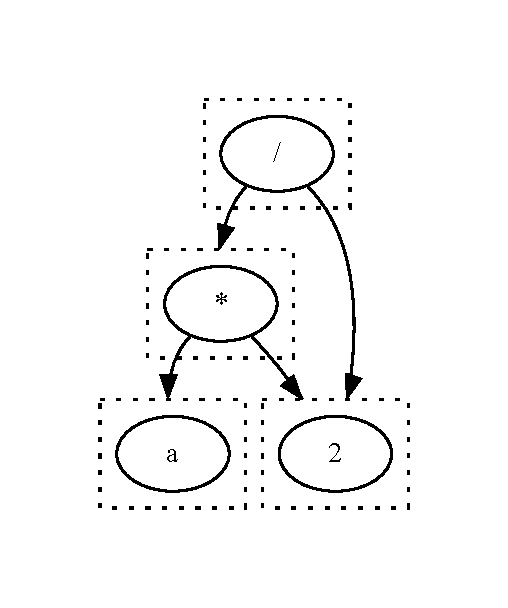
\includegraphics[width=\linewidth, height=4.6cm]{img/egraph1.pdf}
    \caption{}\label{fig:egraph1}
  \endminipage\hfill
  \minipage{0.24\textwidth}
    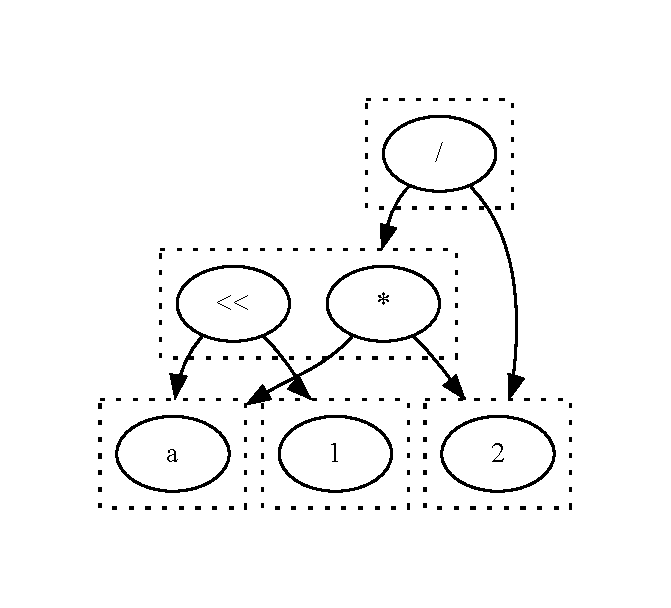
\includegraphics[width=\linewidth, height=4.6cm]{img/egraph2.pdf}
    \caption{}\label{fig:egraph2}
  \endminipage\hfill
  \minipage{0.24\textwidth}%
    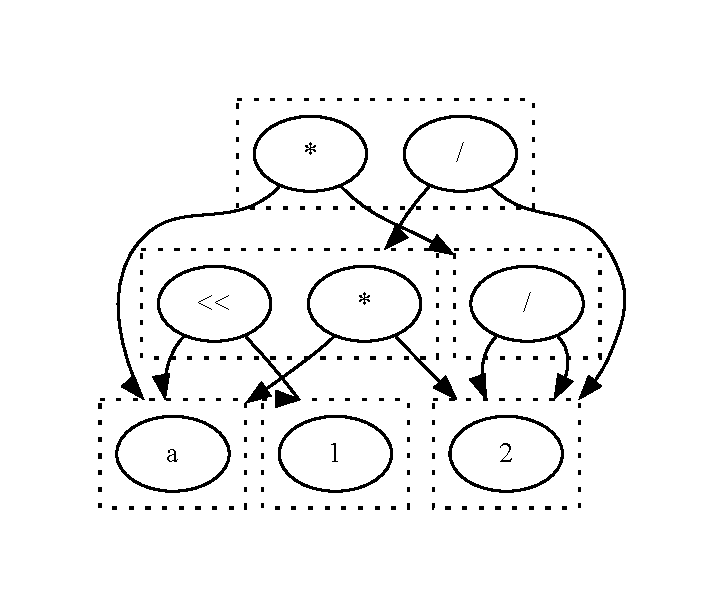
\includegraphics[width=\linewidth, height=4.6cm]{img/egraph3.pdf}
    \caption{}\label{fig:egraph3}
  \endminipage\hfill
  \minipage{0.26\textwidth}
    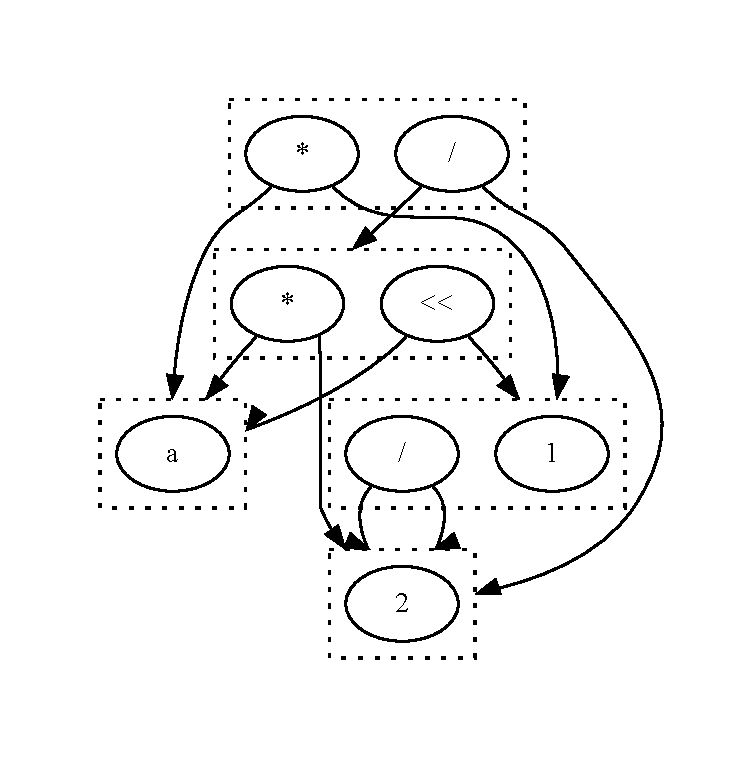
\includegraphics[width=\linewidth, height=4.6cm]{img/egraph4.pdf}
    \caption{}\label{fig:egraph4}
  \endminipage
\end{figure}

When the e-graph is built we can run an equality sturation algorithm. Consider a rewriting system $S$, containing rules of form \texttt{lhs} $\longrightarrow$ \texttt{rhs}, where \texttt{lhs} and \texttt{rhs} are expression in our language. On a high level algorithm does the following: 
\begin{enumerate}
  \item Iterate over rules $r \in S$. For each rule $r$:
  \begin{enumerate}
    \item Try to match the pattern from $r$'s \texttt{lhs} with e-nodes present in the graph. 
    \item If a match was found: if \texttt{rhs} was not present in the graph, add it. Then merge \texttt{lhs} and \texttt{rhs} e-classes.
  \end{enumerate}  
  \item Loop step 1 until each new iteration introduces new equivalences into the graph. After the process is finished, graph is called saturated.
\end{enumerate}

Figures 1--4 illustrate how the algorithm proceeds. In Figure~\ref{fig:egraph2} the rule \texttt{x $\times$ 2 $\longrightarrow$ x $\ll$ 1} was applied. In Figure~\ref{fig:egraph3} the rule \texttt{(x $\times$ y)/z $\longrightarrow$ x $\times$ (y/z)} was applied. In Figure~\ref{fig:egraph4} rules \texttt{x/x $\longrightarrow$ 1} and \texttt{1 $\times$ x $\longrightarrow$ x} were applied.

\newpage
\section{Implementation}
Let us summarize the technical problem and the main components of the developed system. Given a proposition about relations in Coq, we want to prove it using equality saturation, performed by the \texttt{egg} library in Rust. 

A Coq plugin is a tool with external functionality, added to Coq. There are two main approaches of writing Coq plugins: 
\begin{itemize}
    \item \texttt{Ltac}\footnote{\href{https://coq.inria.fr/refman/proof-engine/ltac.html\#ltac}{https://coq.inria.fr/refman/proof-engine/ltac.html\#ltac}} and \texttt{Ltac2}\footnote{\href{https://coq.inria.fr/refman/proof-engine/ltac2.html\#ltac2}{https://coq.inria.fr/refman/proof-engine/ltac2.html\#ltac2}} are languages that help to write simple plugins, combining basic combinations of tactics and actions into a single tactic. It is useful, but not powerful enough to write complex plugins.
    \item The most traditional way of building new complex tactics is to write a Coq plugin in OCaml.
\end{itemize}

Coq's compiler is written in OCaml, so plugins written in OCaml allow to extend Coq's grammar, along with adding complex logic to the tactic, e.g.\ using FFI to call external libraries. To have a better understanding of how all all the components interact with each other in our work, we provide a diagram in Figure~\ref{fig:components}.

\begin{figure}[htbp]
    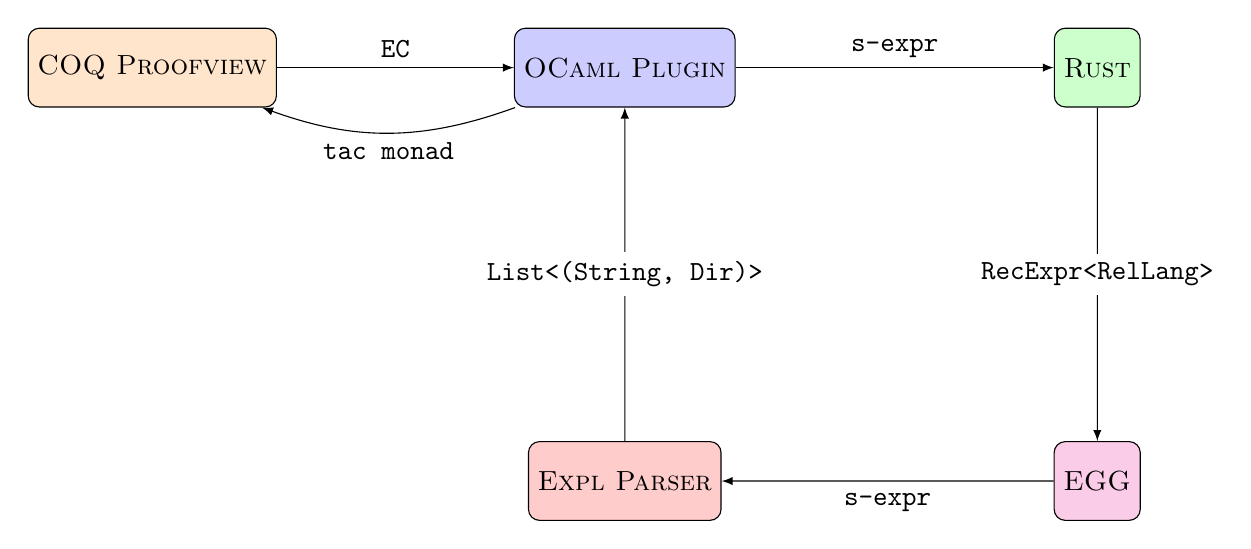
\begin{tikzpicture}[ampersand replacement=\&, scale=1.5]
        \node[rectangle, rounded corners, draw, fill=orange!20, minimum height=1cm] at (0,0) (CP) {\textsc{COQ Proofview}};
        \node[rectangle, rounded corners, draw, fill=blue!20, minimum height=1cm] at (4,0) (OP) {\textsc{OCaml Plugin}};	
        \node[rectangle, rounded corners, draw, fill=green!20, minimum height=1cm] at (8,0) (RUST) {\textsc{Rust}};	
        \node[rectangle, rounded corners, draw, fill=magenta!20, minimum height=1cm] at (8,-3.5) (EGG) {\textsc{EGG}};	
        \node[rectangle, rounded corners, draw, fill=red!20, minimum height=1cm] at (4,-3.5) (EP) {\textsc{Expl Parser}};	

        \draw [-latex] (CP) to node [above, sloped] (TextNode1) {\texttt{EC}} (OP);
        \draw [-latex] (OP) to node [above, sloped] (TextNode1) {\texttt{s-expr}} (RUST);
        \draw [-latex] (RUST) to node [fill=white] (TextNode1) {\texttt{RecExpr<RelLang>}} (EGG);
        \draw [-latex] (EGG) to node [below, sloped] (TextNode1) {\texttt{s-expr}} (EP);
        \draw [-latex] (EP) to node [fill=white] (TextNode1) {\texttt{List<(String, Dir)>}} (OP);
        \draw [-latex] (OP) to[bend left=20] node [below] (TextNode1) {\texttt{tac monad}} (CP);

    \end{tikzpicture}
    \caption{Components of the system}\label{fig:components}
\end{figure}

Data types over each arrow from Figure~\ref{fig:components} will be discussed in detail in the following chapter.  

\subsection{Vernacular Commands}
To extend Coq's grammar with a new tactic or command, one should write a \texttt{.mlg} file, where the tactic's syntax is defined. Consider an example: 

\vspace{0.5cm}
\begin{lstlisting}[language=ocaml_vernac, label=lst:mlg_example]
    DECLARE PLUGIN "coq-via-egg-plugin.plugin"

    VERNAC COMMAND EXTEND cegg_config CLASSIFIED AS QUERY
    | [ "Cegg" "config" reference(r) ] -> { ... } 
    END

    TACTIC EXTEND cegg_solve
    | [ "Cegg" "solve" ] -> { ... } (* Paring and interpretation rule *)
    END
\end{lstlisting}

In listing~\ref{lst:mlg_example}, we define a command called \texttt{cegg\_config} and a tactic called \texttt{cegg\_solve}. A command is marked as \texttt{QUERY}, meaning it is a \textit{pure} function. Otherwise it would have been marked as \texttt{SIDEFF}. 
\begin{definition}[Pure function]
    A pure function is a function where the return value is only determined by its input values, without observable side effects. 
\end{definition}
After the \texttt{|} symbol, we define the parsing rule and the the interpretation rule, separated by \texttt{->}. The parsing rule itself is a set of terminals that are matched against a string of tokens. The interpretation rule is a function that is called when the parsing rule is matched. More on the \texttt{.mlg} file format can be found in the Coq's plugin guide~\footnote{\href{https://github.com/coq/coq/blob/master/doc/plugin\_tutorial/tuto2/src/g\_tuto2.mlg}{https://github.com/coq/coq/blob/master/doc/plugin\_tutorial/tuto2/src/g\_tuto2.mlg}}.

\subsection{OCaml plugin}
When our tactic is called from inside the Coq proof, firstly, we need to extract the goal. Consider an example: 

\vspace{0.5cm}
\begin{lstlisting}[language=coq]
Lemma example (r : relation A) : 
    r^* ;; r^? (@\equiv@) r^*.
Proof.
    Cegg solve eq. 
\end{lstlisting}

When we enter the interactive proof process, we see the following proof state: 

\vspace{0.5cm}
\begin{lstlisting}[language=coq]
    A : Type 
    r : relation A
    ============================
    r^* ;; r^? (@\equiv@) r^*
\end{lstlisting}

Current hypothesises are located above the line and the conclusion of the goal --- below. To interact with Coq from OCaml, we use the Coq-Api\footnote{\href{https://coq.github.io/doc/V8.16.0/api/coq-core/index.html}{https://coq.github.io/doc/V8.16.0/api/coq-core/index.html}}, which provides a widest functionality. To extract that information about the goal in OCaml we first enter the Proofview monad.

\begin{definition}[Monad]
    Monads serve as a representation of computations. Consider a computation to be similar to a function that transforms an input to an output, but with an additional component. This component represents the effect that the function has as a consequence of being executed.
\end{definition}

In the following function \texttt{t} denotes the goal. \texttt{enter} applies the goal-dependent tactic, with \texttt{(t -> unit tactic)} type in each goal independently. 

\vspace{0.5cm}
\begin{lstlisting}[language=ocaml]
    val enter : (t -> unit tactic) -> unit tactic
\end{lstlisting}

Now we see that our tactic, all in all, should be a function that takes goal (\texttt{Proofview.Goal.t}) as input and return a tactic monad (\texttt{unit tactic}). When we have such a function, \texttt{enter} will apply it to each goal. 

Having a \texttt{gl {:} Proofview.Goal.t} as input, we need to split it into the conclusion, hypotheses and the environment, using functions \texttt{concl}, \texttt{hyps} and \texttt{env} respectively. The most import for us is the \texttt{concl}, which we will get. It has a \texttt{EConstr.constr}, which is the most important datatype in Coq, namely the kernel term. It is used to represent expressions, which are built using a set of constructors that correspond to the different types and operations. 

% TODO: Жидокато в конце написал, надо лучше
Our next task is to prepare the conclusion for the \texttt{egg} use. \texttt{Econstr.t} (similar to \texttt{Econstr.constr}) has a huge list of constructors, but we are not expecting to handle most of them. For example, constructors such as \texttt{Forall} or \texttt{LetIn} are not something we expect to see in a proposition about relations. From the limitations of what kind of rules we can pass to \texttt{egg} we can infer that we want to handle particular relations and various operations on them, i.e.\ applications of functions. Moreover, after analysing the Hahn library and the imm code base, we have decided to add some concrete relations as constants: An empty relation, denoted as \texttt{(fun\_ \_ => False)}, which means that for any two elements of the given set are related, and a full relation, denoted as \texttt{(fun \_ \_ => True)}. Thereby the constructors we are interested in are as follows: 

\vspace{0.5cm}
\begin{lstlisting}[language=ocaml]
    type Econstr.constr = 
        | App of 'constr * 'constr array
        | Var of Names.Id.t
        | Lambda of Names.Name.t Context.binder_annot * 'types * 'constr
        | Ind of Names.inductive * 'univs (* Inductive constructors, e.g. True or False *)
\end{lstlisting}

\texttt{Econstr.t} is parsed into a smaller type, which will be then transferred to \texttt{egg}. If unexpected constructors occur in the expression, exception is raised and a error is shown to the user. Data type is an s-expression over strings, with an addition of lambdas: 

\vspace{0.5cm}
\begin{lstlisting}[language=ocaml]
    type goal_s_expr =
        | Symbol of string
        | Application of string * goal_s_expr list
        | Lambda of goal_s_expr * goal_s_expr
\end{lstlisting}

Next step is to pass an object of type \texttt{goal\_s\_expr} to Rust for further processing. We use the \texttt{ocaml-rs}~\cite{OCaml_rust_ffi} Rust library to set up communication between OCaml and Rust. Similar type as \texttt{goal\_s\_expr} is defined in Rust: 

\vspace{0.5cm}
\begin{lstlisting}[language=rust, style=colouredRust]
    pub enum GoalSExpr {
        Symbol(String),
        Application(String, LinkedList<GoalSExpr>),
        Lambda(Box<GoalSExpr>, Box<GoalSExpr>),
    }
\end{lstlisting}

\subsection{Using Egg}





\setmonofont[Mapping=tex-text]{CMU Typewriter Text}
\printbibliography{}
\end{document}
